 \documentclass [12pt]{article} 

\usepackage {amsmath}
\usepackage {amsthm}
\usepackage {amssymb}
\usepackage {graphicx} 
\usepackage {float}
\usepackage {multirow}
\usepackage {xcolor}
\usepackage [ruled,vlined,commentsnumbered,titlenotnumbered]{algorithm2e} \usepackage {array} 
\usepackage {booktabs} 
\usepackage {url} 
\usepackage {parskip} 
\usepackage [margin=1in]{geometry} 
\usepackage [T1]{fontenc} 
\usepackage {cmbright} 
\usepackage [many]{tcolorbox} 
\usepackage [colorlinks = true,
            linkcolor = blue,
            urlcolor  = blue,
            citecolor = blue,
            anchorcolor = blue]{hyperref} 
\usepackage {enumitem} 
\usepackage {xparse} 
\usepackage {verbatim}
\usepackage{algpseudocode}
\usepackage{listings}
\usepackage{xcolor}
\lstset { %
    language=C++,
    backgroundcolor=\color{black!5}, % set backgroundcolor
    basicstyle=\footnotesize,% basic font setting
}
\newtheorem{theorem}{Theorem}
\newtheorem{remark}{Remark}
\newtheorem{lemma}[theorem]{Lemma}
\newtheorem{corollary}[theorem]{Corollary}
\theoremstyle{definition}
\newtheorem{definition}{Definition}[section]
\newtheorem{claim}{Claim}
\newtheorem{proposition}{Proposition}






\DeclareTColorBox {Solution}{}{breakable, title={Solution}} \DeclareTColorBox {Solution*}{}{breakable, title={Solution (provided)}} \DeclareTColorBox {Instruction}{}{boxrule=0pt, boxsep=0pt, left=0.5em, right=0.5em, top=0.5em, bottom=0.5em, arc=0pt, toprule=1pt, bottomrule=1pt} \DeclareDocumentCommand {\Expecting }{+m}{\textbf {[We are expecting:} #1\textbf {]}} \DeclareDocumentCommand {\Points }{m}{\textbf {(#1 pt.)}} 

\begin {document} 

\vspace {1em} 
\begin {Instruction} 
Adapted From Virginia Williams'lecture notes.
\end {Instruction}  

{\LARGE \textbf {COMP 285 (NC A\&T, Spr `22)}\hfill \textbf {Lecture 33} } 

\begin{centering}
\section*{Max Flows and Mininum Cuts}
\end{centering}


\section{Formulation of the Maximum Flow Problem}

You are given an input graph $G = (V, E)$, where the edges are directed. There is a function $c : E \to R\geq 0$ that defines the capacity of each edge. We also label two nodes in $G$, $s$ and $t$, as the source and destination, respectively. The task is to output a flow of maximum value. We will shortly define what a flow is and what a flow of maximum value means. 

A flow $f$ is a function $f : E \to R\geq 0$ such that 
\begin{enumerate}
    \item Capacity constraints are satisfied: 
    $$
        \forall (u, v ) \in E : 0 \leq f (u, v ) \leq c(u, v )
    $$. 
    \item Flow conservation constraints are satisfied: 
    $$
    \forall v \in V \setminus \{s, t\} : \sum_{x \in N_{\text{in}}(v)} f (x, v ) = \sum_{y\ in N_{\text{out}}(v)} f (v, y )
    $$
    Here $N_{\text{in}}(v )$ denotes the set of nodes with an edge that points to $v$ and $N_{\text{out}}(v )$ denotes the set of nodes that $v$ points to.
\end{enumerate}

\begin{figure}[h!]
    \centering
    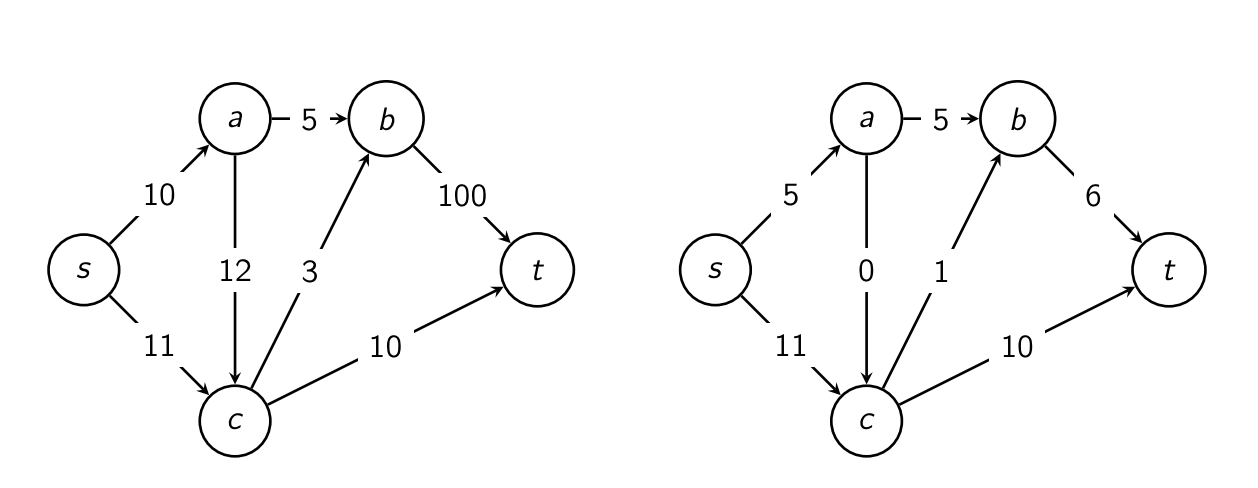
\includegraphics[scale=0.6]{max_flow_ex.png}
    \caption{(Left) Graph $G$ with edge capacities (Right) Graph $G$ with a sample flow.}
    \label{fig:max_flow_ex}
\end{figure}
 

Suppose that there are no edges going into $s$ and no edges coming out of $t$. From the above, you can verify yourself that $\sum_{x \in N_{\text{out}}(s)} f (s, x) = \sum_{y \in N_{\text{in}}(t)} f (y, t)$. We define the value $x \in N_{\text{out}}(s) f (s, x)$ to be the value of the flow $f$ . We usually denote the value of a flow $f$ as $|f |$. If there are edges going into $s$ and out of $t$, then the value of $f$ is $$
|f | = \sum_{x \in N_{\text{out}}(s)} f (s, x) - \sum_{ y \in N_{\text{in}}(s)} f (y, s)
$$.

The max flow problem is to find some flow f such that $|f |$ is maximized. Remark 1. In the analysis below we consider graphs with a single source s and a single sink t. However, if we need to work with a graph with multiple sources, we can do so by adding a new source node, and then adding edges with capacity infinity from it to each of the multiple sources. Similarly, if we want to have multiple sinks, we add a new sink node and add edges from the multiple sinks to that sink with capacity infinity.

\section{Example}

In Fig. \ref{fig:max_flow_ex}, we have a graph $G$ and a sample flow $f$ . Observe that the two constraints for a flow are satisfied. There can be multiple other flows possible that can satisfy the constraints. For our given flow, $|f | = 16$. The max flow for this graph is actually $18$, as we will see shortly.


\section{Formulation of the Minimum Cut Problem}

Now, we give a formulation of the min cut problem defined for directed graphs with source and destination nodes $s$ and $t$. Note that there is also a version of the min cut problem without a source and sink node, though we won't discuss that now. An s-t cut is a partition $V = S \cup T$ where $S$ and $T$ are disjoint and $s \in S, t \in T$, and the size/cost of an s-t cut is $c(S, T) := \sum_{x\in S, y\in T} c(x, y )$.

For our graph $G$ shown above, if we set$ S = \{s, a, c\}$ and $T = \{b, t\}$, then the cost of the cut is $c(a, b) + c(c, b) + c(c, t) = 5 + 3 + 10 = 18$. If we take another cut $S
' = \{s, c\}, T' = \{a, b, t\}$, then $c(S', T') = c(s, a) + c(c, b) + c(c, t) = 10 + 3 + 10 = 23$. Note that we do
not consider the edge $\{a, c\}$ as it is in the wrong direction (we only consider edges from $S'$ to $ T'$).


\section{The Max-Flow Min-Cut Theorem}

\begin{lemma}
For any flow $f$ and any s-t cut $(S, T)$ of $G$, we have $|f | \leq c(S, T)$. In particular,the value of the max flow is at most the value of the min cut.
\end{lemma}

\begin{proof}

\begin{align*}
|f| &= \sum_{x \in N_{\text{out}}(s)} f(s,x) - \sum_{y \in N_{\text{in}}(s)} f(y,s) \\
&=\sum_{v \in S} \left(\sum_{x \in N_{\text{out}}(v)} f(v,x) - \sum_{y \in N_{in}(v)} f(y,v) \right) \tag{by flow conservation constraing for $v \neq s$} \\
&=\sum_{v \in S} \left(\sum_{x \in N_{\text{out}}(v) \cap S} f(v,x) - \sum_{y \in N_{in}(v) \cap S} f(y,v) \right) + \sum_{v \in S} \left(\sum_{x \in N_{\text{out} \cap T}(v)} f(v,x) - \sum_{y \in N_{in}(v) \cap T} f(y,v) \right) \\
&=\sum_{v \in S} \left(\sum_{x \in N_{\text{out} \cap T}(v)} f(v,x) - \sum_{y \in N_{in}(v) \cap T} f(y,v) \right) \tag{first term sums to $0$} \\
&\leq \sum_{v \in S, x \in T, x \in N_{\text{out}}(v)} f(v,x) \\
&=\leq \sum_{v \in S, x \in T, x \in N_{\text{out}}(v)} c(v,x) \\
&= c(S,T)
\end{align*}

In the proof, $\sum_{v \in S} \left(\sum_{x\in N_{\text{out}}(v)} f(v,x) - \sum_{y\in N_{\text{int}}(v)} f(y,v)\right) = 0$ since we add and subtract the flow $f (u, v )$ for every $u, v \in S$ such that $(u, v ) \in E$.
\end{proof}

We get the following consequence.

\begin{corollary}
If we can find $f$ and $(S,T)$ such that $|f| = c(S,T)$ then $f$ is a max-flow and $(S,T)$ is a min s-t cut.
\end{corollary}

It turns out we can always find such an $f$ and $(S,T)$ for any graph.

\begin{theorem}{Max-Flow Min-cut Theorem}
For any graph $G$, source $s$ and destination $t$, the value of the max flow is equal to the cost of the min cut
\end{theorem}

We will show this by coming up with an algorithm. The algorithm will take the graph $G$ and some flow $f$ that has already been constructed, and create a new graph that is called the residual graph. In this new graph, the algorithm will try to find a path from s to t. If no such path exists, we will show that the value of the flow we started with is the value of the maximum flow. If not, we show how to increase the value of our flow by pushing some flow
on that path.

\begin{figure}[h!]
\centering
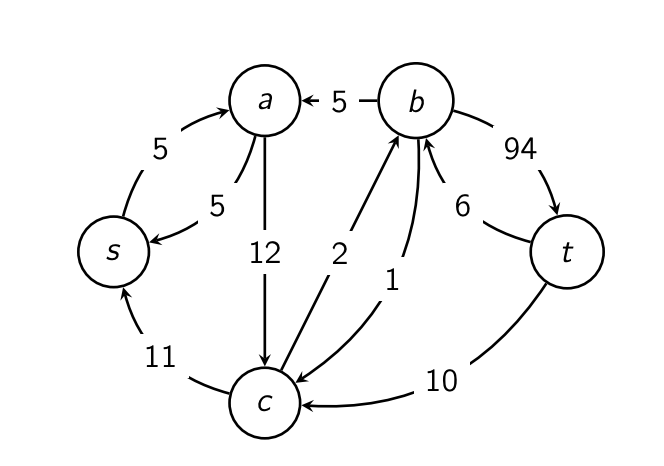
\includegraphics[scale=0.6]{max_flow_res.png}
\caption{The Residue network given the flow presented in Figure \ref{fig:max_flow_ex}}
\label{fig:max_flow_res}
\end{figure}


\section{The Ford-Fulkerson Max-Flow Algorithm}

We will make an assumption on our graph. The assumption can be removed, but it will make our lives easier. We will assume that for all $u, v \in V$ , $G$ does not have both edges $(u, v )$ and $(v, u)$ in $E$. We can make this condition hold by modifying the original graph in the following way. If $(u, v ), (v, u) \in E$, we split the edge $(u, v )$ to two edges $(u, x)$ and $(x, v )$, where $x$ is a new node we introduce into the graph. This makes the number of nodes at most $m + n$. 

Now, let $f$ be a flow given to us. We will try to see if we can improve this flow. We will define the residual capacity $c_f : V \times V \to R_{\geq 0}$ as follows. 

$$
c_f (u, v ) = \begin{cases}
    c(u, v ) - f (u, v ) & \text{if }(u, v ) \in E \\
    f (v, u) & \text{if }(v, u) \in E \\
    0 & \text{ otherwise. }
\end{cases}
$$

Basically, what this does is that, if there is any flow through the edge, you remove the flow from the capacity and add an edge in the opposite direction with the value of the flow. The reason we do this is because the flow we picked thus far might not be the correct flow, and this formulation allows us to undo changes that we have done through ``adding flow'' in the revere direction. The residual capacity $c_f (u, v )$ represents how much flow we can send from $u$ to $v$ in addition to the flow $f$. 

We define $G_f$ to be a residual network defined with respect to $f$ , where $V (G_f ) = V (G)$ and $(u, v ) \in E(G_f )$ if $c_f (u, v ) > 0$. Figure \ref{fig:max_flow_res} shows $G$ with the residual edges. We will show that, if there is a path from $s$ to $t$ in $G_f$ , then $f$ is not a max flow. If no such path exists, that $f$ is a max flow.


\begin{lemma}
If $t$ is not reachable from $s$ is $G_f$ , then $f$ is a maximum flow.
\end{lemma}
\begin{proof} 
Let $S$ be the set of nodes reachable from $s$ in $G_f$ and $T = V \setminus S$. There are no edges in $G_f$ from $S$ to $T$ since the nodes in $T$ are not reachable from $s$. Note that $(S, T)$ defines an $s-t$ cut. Now consider any $v \in S, w \in T$. We have $c_f (v, w) = 0$ since $(v, w)$ is not an edge in $G_f$ . There are three cases: 
\begin{enumerate}
    \item If $(v, w) \in E$, then by definition $c_f (v, w) = c(v, w) - f (v, w) = 0 \implies c(v, w) = f (v, w)$\item If $(w, v ) \in E$, then $c_f (v, w) = f (w, v ) = 0$.
    \item If $(v, w) \notin E and (w, v ) \notin E$, we can disregard $(v, w)$ and $(w, v )$ since they do not appear in any flow or cut.
\end{enumerate}

 Using this, and the proof in Lemma 2, we have 
 \begin{align*}
 |f | &= \sum_{v\in S} \left( \sum_{x\in N_{\text{out}(v)} \cap T} f (v, x) - \sum_{y\in N_{\text{in}}(v) \cap T} f (y, v ) \right) \\
 &= \sum_{v\in S} \sum_{x\in N_{\text{out}(v)} \cap T} f (v, x) \tag{from case 2 the second term is 0} \\
 &= \sum_{v\in S} \sum_{x\in N_{\text{out}(v)} \cap T} c(v, x) \tag{from case 1}\\
 &= c(S, T)
 \end{align*}

 Thus, we show that the flow is equal to the cut. From Corollary 3 we know that $f$ is a maximum flow, and $(S, T)$ is a min cut.
\end{proof}


\begin{lemma}
If $G_f$ has a path from $s$ to $t$, we can modify $f$ to $f'$ such that $|f | < |f'|$.
\end{lemma}
\begin{proof}

Pick a path $P$ from $s$ to $t$ in $G_f$ , and consider the edge of minimum capacity on the path. Let that capacity be $F$ . Then we can increase our flow by $F$ . For each edge in $P$, if $c_f (v, w)$ is the right direction (i.e., there is an edge $(v, w) \in E(G)$), then we can increase our flow on this edge by $F$ . If $c_f (v, w)$ is in the opposite direction (i.e., $(w, v ) \in E(G)$), then we can decrease the flow on this edge by $F$ . In effect, we are ``undoing'' the flow on this edge. By doing so, we have increased our flow by $F$. 

As an example, consider Fig. \ref{fig:max_flow_res} again. The path $s \to a \to c \to b \to t$ is a path with minimum capacity $2$. Therefore, we can update our flow and push additional $2$ units of flow, resulting in a flow of $18$. 

Formally, Let $s = x_0 \to x_1 \to ... \to x_k = t$ be a simple path $P$ in $G_f$ , and let $F = \min_i c_f (x_i , x_{i+1})$. Define a new flow $f'$ where 
$$
f' (u, v ) = \begin{cases}
    f (u, v ) + F & \text{ if }(u, v ) \in P\\
    f (u, v ) - F & \text{ if }(v, u) \in P \\
    f (u, v ) & \text{ otherwise }.
    \end{cases}
$$

We now need to show that $f'$ is a flow. The capacity constraints are satisfied because for every $(u, v ) \in E$,
\begin{enumerate}
    \item If $(u, v ) \in P$, then $0 \leq f (u, v ) + F \leq f (u, v ) +c_f (u, v ) = f (u, v ) +c(u, v )-f (u, v ) = c(u, v )$. 
    \item If $(v, u) \in P$, then $f (u, v ) - F \leq f (u, v ) \leq c(u, v )$ and $f (u, v ) - F \geq f (u, v ) - c_f (v, u) = 0$.
    \item Otherwise, $f (u, v )$ is from the original flow $f$ .
\end{enumerate}

The conservation constraints are also satisfied: Recall that $P$ is a simple path. Thus, for every $v \in V \setminus \{s, t\}$, $P$ uses $0$ or two edges incident on $v$ . If $P$ uses $0$ edges on $v$, then flow values of the edges incident on $v$ have not changed when going from $f$ to $f'$ . Thus, suppose that $P$ uses two edges $(x, v )$ and $(v, y )$ incident on $v$. Because in $G_f$ some edges appear in the opposite direction compared to $G$, we need to consider a few cases. 

\begin{enumerate}
    \item $(x, v )$ and $(v, y )$ are both in the same direction (an edge into $v$ and an edge out of $v$ ); the flow into $v$ increases by $F$ and the flow out of it also increases by $F$ .
    \item $(x, v )$ and $(v, y )$ are both in the opposite direction $((v, x), (y, v ) \in E$); the flow into $v$ decreases by $F$ and the flow out of it also decreases by $F$ .
    \item $(x, v )$ is in the correct direction and $(v, y )$ is in the opposite direction. Then the flow into $v$ changes by $F - F = 0$.
    \item $(x, v )$ is in the opposite direction and $(v, y )$ is in the correct direction. Then the flow out of $v$ changes by $F - F = 0$. 
\end{enumerate}

Finally, note that we increase our flow by $F$ . Consider the edge $(s, x_1)$ in $P$. If $(s, x_1) \in E$, the flow out of $s$ increases by $F$ . If $(x_1, s) \in E$, the flow into s decreases by $F$ . By our definition of $G_f$ , it must be that $F > 0$, and we get that $|f'| > |f |$. 
\end{proof}

From this, we can construct an algorithm to find the maximum flow. Starting with some arbitrary flow of the graph, construct the residual network, and check if there is a path from $s$ to $t$. If there is a path, update the flow, construct the new residual graph and repeat. Otherwise, we have found the max flow. 

A path from $s$ to $t$ in the residual graph is called an augmenting path, and pushing flow through it to modify the current flow is referred to as augmenting along the path. 

The run time of this algorithm is bounded by the number of times we update our flow. If the edge capacities are all integers, we can increase the flow by at least 1 each time we update our flow. Therefore, the runtime is $O(|f |m)$ where $|f |$ is the value of the max flow. If we have rational edge capacities, then we can multiply all edge capacities by a factor to make them all integers. However, the runtime blows up by that factor as well. If we have irrational edge capacities, then the algorithm is no longer guaranteed to terminate. So we have a problem.

\begin{algorithm}
\caption{maxflow($G,s, t$)}
\label{alg:maxflow_algorithm}
\begin{algorithmic}
\State $f \gets$ all zeros flow
\State $G_f \gets G$
\State \While{$t$ is reachable from $s$ in $G_f$ (check using DFS/BFS)}{
    \State $P \gets$ path in $G_f$ from $s$ to $t$ 
    \State $F \gets$ min capacity on $P$
    \State $f \gets f'$ as defined in Lemma 5 above.
    \State Update $G_f$ to the corresponding new flow.
}
\State \Return $f$
\end{algorithmic}
\end{algorithm}
 

We will save the day in the next sections. Algorithm \ref{alg:maxflow_algorithm} is called the Ford-Fulkerson method.

It is actually part of a family of algorithms that depend on how the path $P$ between $s$ and $t$ in $G_f$ is selected. One can obtain $P$ via DFS, BFS, or any other method for selecting paths. It turns out that two methods work particularly well: the shortest path method and the fattest path method. The shortest path method is known as the Edmonds-Karp algorithm or Dinic's algorithm. 

\textbf{The fattest path method.} This method finds a path between $s$ and $t$ that maximizes $\min_{e \in P} c_f (e)$ among all $s-t$ paths $P$. Finding such a path can be done in $O(m + n)$ time by a clever mix of linear time median-finding and $DFS$. 


\textbf{The shortest path method (the Edmonds-Karp algorithm/Dinic's algorithm)}. This method picks the path between $s$ and $t$ using BFS, thus picking a path that minimizes the number of edges. Finding such a path also runs in $O(m)$ time: BFS takes $O(m + n)$ to explore the whole graph, but since we only care about the vertices reachable from $s$ this is $O(m)$ time. 

Since both methods of selecting a path run in linear time, the main question becomes, how many iterations does Ford-Fulkerson perform? We will answer these questions below in the next section.




































\end{document}